\documentclass{l4proj}

\usepackage{url}
\usepackage{fancyvrb}
\usepackage[final]{pdfpages}
\usepackage[acronym,toc]{glossaries}
%\usepackage[toc]{glossaries}
\newcommand{\tex}{\TeX}
\newcommand{\BibTeX}{B{\sc ib}\TeX}
\newcommand{\bibtex}{\BibTeX}
\newcommand{\latex}{\LaTeX{} }
\newcommand{\revisit}{\#\#\#}

\makeindex
\makeglossaries

%						Short plural key				 Long plural key
\newacronym[\glsshortpluralkey=smpls,\glslongpluralkey=samples]{smpl}
%key		 value
{SAMPLE}{Sample entry}

\newglossaryentry{sample}{name={sample}, description={a sample glossary entry}}
% ==========================================
% 	Acronyms 				
% 				  key  		displayed		Full stringaod
\newacronym{ajax}		{AJAX}			{Asynchronous JavaScript And XML}
\newacronym{aod}		{AOD}				{Architecture Overview Diagram}
\newacronym{asp}		{ASP}				{Active Server Pages}
\newacronym{bat}		{BAT}				{Batch File}
\newacronym{case}		{CASE}			{Computer-Aided Software Engineering}
\newacronym{ci}			{CI}				{Continuous Integration}
\newacronym{css}		{CSS}				{Cascading Style Sheet}
\newacronym{html}		{HTML}			{HyperText Markup Language}
\newacronym{http}		{HTTP}			{HyperText Transfer Protocol}
\newacronym{id}			{ID}				{Identifier}
\newacronym{ide}		{IDE}				{Integrated Development Environment}
\newacronym{jre}		{JRE}				{Java Runtime Environment}
\newacronym{msdnaa}	{MSDNAA}		{Microsoft Developer Network Academic Alliance}
\newacronym{msss}		{MSSQL}			{Microsoft SQL Server}
\newacronym{msvs}		{MSVS}			{Microsoft Visual Studio}
\newacronym{mvc}		{MVC}				{Model View Controller}
\newacronym{oo}			{OO}				{Object-Oriented}
\newacronym{sql}		{SQL}				{Structured Query Language}
\newacronym{ssh}		{SSH}				{Secure Shell}
\newacronym{svn}		{SVN}				{Subversion}
\newacronym{ui}			{UI}				{User Interface}
\newacronym{uri}		{URI}				{Uniform Resource Identifier}
\newacronym{url}		{URL}				{Uniform Resource Locator}
\newacronym{xml}		{XML}				{eXtensible Markup Language}

% ==========================================
% 	Glossary terms
% 				  			key  	  Name						 Explanation
\newglossaryentry{svntag}	{name={SVN Tag}, 	description={A snapshot of a project in time, saved with a human-readable name}}
\newglossaryentry{unix}		{name = {UNIX},		description={An open-source operating system}}


% ==========================================
% ==========================================
% ==========================================
% ==========================================

\begin{document}
\title{\bibtex{} Entry Manager}
\author{John Lewis Thow [0701068]}
\date{\today}
\maketitle




\begin{abstract}
Abstract for the project\\\\

\revisit
A \gls{sample} entry and \gls{xml}. Second use: \gls{xml}.

Plurals: \glspl{sample}. Reset acronym\glsreset{xml}.
First use: \glspl{xml}. Second use: \glspl{xml}.\glsreset{xml}

\end{abstract}


%\chapter*{Thanks \& Acknowledgements}
\newpage
\section*{Personal Thanks}
\begin{itemize}
\item I'd like to wholeheartedly thank Dr David Manlove for his guidance, assistance \& expertise on this project, as well as his patience \& dedication when it came to other matters;
\item Thanks to Gregg O'Malley for introducing me (\& David) to a different approach to concurrent access to entries;
\item Thanks to all of the volunteers who took part in my evaluation, as well as to Dr Colin Perkins for his assistance in organising the sessions, during which some of the evaluations took place;
\item I'd like to give Graham Mooney a mention for his DIV-ine tutorial;
\item Thomas Anderson of the Amor Group;
\item I'd like to thank my family, friends and classmates for all of their support;
\item Finally, I'd like to give a very warm thank you to all of the staff in the School (Department!) of Computing Science at the University of Glasgow, both retired \& active who have had an input on my education over the past 4 years.
\end{itemize}
\section*{Acknowledgements}
I'd also like to mention some other parties who have (perhaps indirectly) had a positive impact on the project: \
\begin{itemize} 
\item Microsoft - in particular for their Academic Alliance (MSDNAA) programme, as well as for the .NET framework and the C\# programming language;
\item The NUnit Community for their test framework;
\item The NHibernate Community;
\item ThoughtWorks for making their Continuous Integration software open-source;
\item SourceForge for hosting the Subversion repository on which the project was hosted, along with bug tracking software;
\item The Stack Overflow community for their extensive knowledge base and source of ideas;
\item kryogenix.org for their table sorting JavaScript library `sorttable';
\item JetBrains for their Visual Studio productivity plug-in `ReSharper';
\item The Dynamic Drive (DHTML) community.
\end{itemize}

\educationalconsent
%
%NOTE: 	if you include the educationalconsent (above) 
% 			and your project is graded an A then
%      	it may be entered in the CS Hall of Fame
%
\tableofcontents
%==========================================================
\chapter{Introduction}
\label{intro}
Discuss the intention of the intro \& its contents.

\section{Preliminaries}
\subsection{\TeX{}}
In the words of its creator, \TeX{} is ``a [new] typesetting system intended for the creation of beautiful books---and especially for books that contain a lot of mathematics'' \cite{DK84}.  The \TeX{} program is a set of primitive commands for basic typesetting, and also allows users to create more complex commands in terms of simpler ones.  Donald Knuth created the \TeX{} program in 1978, a subsequent version of which makes up the core of the program that is used today \cite{TeXOrigin}.  The use of \TeX{} to its potential requires that one has had considerable experience with programming techniques; it is as a result of this that the use of \TeX{} on its own is left to typography and programming professionals \cite{KD95}.

\subsection{\LaTeX}
\latex was created by Leslie Lamport in 1985, to allow one to exploit the powerful features of \TeX{} without first having to familiarise oneself with programming techniques. \latex contains a range of commands written in terms of primitive \TeX{} commands, providing users with a set of higher-level commands for the production of complex documents.  It also allows for a separation of concerns between the information that is being presented from the formatting that has to be applied when publishing \cite{KD95}.

\subsection{\bibtex}
It is standard to find a bibliography at the end of a scientific publication. \latex provides an `environment'\footnote{An environment is used to specify an area of a document where the text has to be presented with different indentation, line width, typeface and so on \cite{KD95}.  The environment used by \latex is called `\texttt{thebibliography}'.} which allows bibliographic references to be listed and stored in one area of a document \cite{KD95}, but this approach requires that each document has its own list of references, which may lead to redundancy and inconsistency if, for example, an author has multiple publications on the same subject. 

\bibtex{} is an auxiliary program to \latex which provides the authors with the ability to store all of their bibliographic references in one or more files.  Each reference, or `entry', is uniquely identified by its cite key, which is used within a document where the reference is made.\footnote{A reference to a citation is inserted by using the \latex command \texttt{$\backslash$cite\{citeKey\}} in the body of the document, where `citeKey' is the identifier of the reference in one of the referenced bibliographic files}

The benefit of using \bibtex{} as a means of bibliography production is that a file set is easier to maintain than having sporadic files, each with individual collections of references, as one file can be re-used for all publications.

\section{Problem Statement, Aims \& Motivation}
An author may have a vast number of bibliographic references, through having making a large amount of citations over years of work.  The task of managing this library of references is an issue in itself; authors might have clashing cite keys or entries that are recorded twice in the library, for example.  It is also highly important to ensure that field names are not misspelled --- especially when a field is optional, as misspelling a field name results in it being ignored without warning \cite{OP88}.

The problem of managing entries is exacerbated when multiple users collaborating on a piece of work need to share collections of entries: with no management system in place, users have to find a way to consistently distribute files by email and other manual methods, as well as ensuring that there have been no clashing entries.

The main aim of this project is to try to come up with a solution to solve the aforementioned problems.  The project is also undertaken with some lesser, but still important, aims in mind, which are listed presently:
\begin{itemize}
\item develop a good understanding of the technologies used;
\item observe good software engineering practice during development and testing;
\item develop professional attitude and strategy for dealing with project matters;
\item \revisit
\end{itemize}

%it will be important to evaluate both the usability and effectiveness of the product by   \bibtex{} entries for multiple users.

\section{Outline of Report}
%List these as references to each section!
The remainder of this report will discuss how producing a solution to address the problem of managing \bibtex{} references was undertaken. 
\begin{itemize}
\item Chapter~\ref{backgrnd} provides some background information to the project and examines other work and projects that have been carried out to address the problem.
\item Chapter~\ref{reqs} covers the detailed requirements of the project.
\item Chapter~\ref{design} covers the design of the solution to the problem.
\item Chapter~\ref{impl} covers the implementation of the project in detail.
\item Chapter~\ref{testing} covers how the software product was tested.
\item Chapter~\ref{eval} covers evaluations carried out on the project.
\item Chapter~\ref{conclusion} concludes the report with a summary and provides the reader with some ideas for future work in the area.
\end{itemize}

%======================================================

\chapter{Background Survey}
\label{backgrnd}
There have been many projects and programs created to try to tackle to complexities of managing \bibtex{} entries, some of which will be examined herein.  Firstly, some of the criteria for examinations are listed before discussing the examinations, followed by a summary of findings of the examinations to be kept in mind for the rest of the project.

The products that are examined are:
\begin{itemize}
	\item \bibtex{} Entry Manager by Ravi Tez Kota
	\item BiblioScape by CG Information
	\item \bibtex Manager by Mitesh Pravin Furia 
\end{itemize}

\section{Examination Criteria}
The products examined in this section will be judged on several factors, outlined below.

Each assessment will examine how positive qualities are achieved, as well as how shortcomings are encountered, so that lessons can be learned from other products and problematic issues can be avoided.  It is advantageous at this point to mention that evaluations on the final product from this project will include an examination on the same criteria in Chapter~\ref{eval}.
\begin{itemize}
	\item \gls{ui} to the system:
	\begin{itemize}
		\item How well laid out is the \gls{ui}? 
		\item Is it consistent throughout use?
		\item Is it cluttered and complicated or well spaced out and simple?
		\item Is it intuitive to deduce how a user should perform an action and, where it is not, is it easy to get help?
		\item Is it clear when an action has been performed?
		\item Does it have a look and feel that is easy on the user's eyes?
	\end{itemize}
	\item Features of the system:
	\begin{itemize}
		\item Does the system support multiple users? If so, how?
		\item What expected \& basic\footnote{`Basic' functions are defined to be Add, Edit, Delete, Import, Export and Search. These functions were designated `basic' after developing a general understanding of what a reference management system is expected to do at early project meetings with Dr Manlove.} functions are available for the user to perform? Are any missing?  % acceptable?
		\item What further\footnote{`Further' functions are defined to be any function other than those mentioned in footnote 1 (Add, Edit, Delete, and so on.)} functions are available to the user? 
		\item What range of formats are available to import from and export to?
		\item How well documented is the system?
	\end{itemize}
	\item Fault Tolerance/Robustness:
	\begin{itemize}	
		\item How well does the program cope with poorly formatted entries?
		\item How well does it cope with invalid user input?
		\item Is the software free from visible errors and problems?
	\end{itemize}
\end{itemize}

\section{Examinations}
This section contains the examinations of several existing products, both public projects and previous projects undertaken by students in previous years at the University of Glasgow.  Examinations were performed on a laptop running Windows 7 Professional (64-bit edition).

\subsection{\bibtex{} Entry Manager}
The \bibtex{} Entry Manager was developed by Ravi Tez Kota (known as `Ravi'), an M.Sc. student at the University of Glasgow, under Dr Manlove's supervision in 2010.

\subsubsection{Paradigm}
Ravi's project is a web-based reference management system which consists of a database for storage of entries and a web front-end for users to interact with using a web browser.

\subsubsection{Ease of set-up}
In a nutshell, the server side of the product is not convenient to set-up.  The user must have an instance of MySql server running on the machine from which they'd like to serve pages; they must ensure that Apache Tomcat is installed as a page rendering server; and they must have a Java Runtime Environment (JRE) installed.  The installers for each of these products were included with the content of the product, though that did not greatly reduce the effort required to set them up.  Following set-up of components, the user must set up the database using a provided \gls{sql} script and finally add the files in the `bibtex' directory to Apache Tomcat's content directory.  

This may be a lengthy process, but it only has to be done once per instance of the system, which works in its favour. If the system were set up at a central location, many people could log on to the system at once by visiting a \gls{url}, which would give end-users a very simple method of access without involving them in the set up process (as intended with a web-based product).

\subsubsection{Examination of product}
After installation, the program is easy to navigate to; the user simply points their web browser to the \gls{url} and the initial page is loaded. The system supports different users by way of a registration and log-in process, authenticated with a user name (email address) and password combination.

The sign-up and log-in pages are simple and consistent in terms of layout, but after logging in the look and feel of the site changes.  This is useful in terms of letting the user know that they are authenticated, but it means that one must re-acquaint oneself with the new layout before performing any actions.  Reducing this extra burden in terms of cognitive load would be advantageous in a new system.

The product has two navigation areas which contain different sets of commands in different orders. 
In setting out to perform this background research, it was intended that the examiner would upload/open a file and perform further additions, modifications, deletions and searches across known entries from that initial file.  The lack of file import capability in Ravi's Bibtex Entry Manager was somewhat limiting to the consistency of the examination on this product, and was a significant shortcoming of the product. 

It is easy to deduce from the homepage what a user should click to add an entry to the system, though after an addition is performed, no message is shown to indicate success or failure of the operation.  It is clear that Nielsen's first heuristic\footnote{\label{nielsenH1} Nielsen's first heuristic says that the system should always keep users informed about what is going on. (Visibility of system status) \cite{NielsenHeuristics}} should be adhered to when designing future solutions to this problem.% don't think it is sufficient just to cite this web page, though they are listed here: http://www.useit.com/papers/heuristic/heuristic_list.html

After a break of perhaps twenty minutes in the examination, the user returned and reloaded the home page of the project, only to find that an error had occurred (a NullPointerException was thrown, resulting in a \gls{http} 500 error).  The error was not dealt with in a user-friendly fashion and shows the product in an unprofessional light.  The lesson to be learned here is that the product should deal with errors in a professional manner and not show exceptions on screen to users.

There is no provided `export' functionality, so items cannot be taken out of the system and used directly in the \bibtex{} environment without first reconstructing the entry.  This is quite inconvenient for a user; the lesson to be learned from this is that basic functionality should be provided to ensure that the system is useful to a user.
The modification of an entry is relatively straightforward, although if a user wishes to change an entry's type after it has been saved to the database they will be disappointed, as the entry type is not a field that can be changed by any visible means without re-creating it in the database.

Searching is a bit of a mystery with this product; it is difficult to deduce what state a search is in, given that there is no feedback to the user to say that a search is ongoing, complete, or otherwise.  This lack of feedback makes  for a confusing experience with search and adds to the call for future projects and solutions to adhere to Nielsen's first heuristic. Unfortunately, there is no visible help menu or area to the product to help to describe how any of the functions behave, which is something that would have been particularly helpful to assist with the search function\footnote{Again, Nielsen covers this in his list of heuristics.}.  This lack of help or support is a shortcoming of the product and future projects should provide to avoid usability issues.

There is a provision for users to be able to switch to another database server from the one that they are using.  This might be helpful to some users, but there is potential for unnecessary replication across multiple servers.  It is also unclear from the user interface what database engines and schemas are supported by the system, which is another point that should be well covered by a user manual or help system.

Entries can be categorised by users into different groups.  This involves creating a group with a name and a description, changing to the new group and then adding entries to the group by the method previously used.  This is a helpful feature for categorising entries that do not yet exist, but a limitation of the system is that entries cannot be transferred from one group to another, and it means that they cannot belong to more than one group at any time.  Any future system implementing a grouping capability should allow entries to belong to many groups and should allow modification at any stage after addition to the set of entries, rather than restricting the flexibility of the system by failing to provide the functionality to make these changes.

The site allows users to access the same set of entries at the same time.  The issue that arises from this is that users may make changes to the same entry simultaneously.  Ravi's solution deals with the problem by locking an entry until the first user to access it saves any changes they have made, or exits the viewing window.  This is a neat solution and means that there can be no overlapping of interests when multiple people access the same entry.  An issue that arises from this method is that if one user (A) views an entry, then forgets to close the window, the entry is locked for a period of time.  When users B and C come to view it (perhaps with no intention of modifying it), they find that they cannot, leaving them unable to work and potentially frustrated while the time period of user A's viewing expires or they leave the window.

\subsection{BiblioScape}
BiblioScape is a desktop-based bibliographic data and note collection suite produced by CG Information.  It was created with the aim to ``build first class bibliographic software for the 21st century''.  It contains many tools which shall not be included in this examination as they are deemed to be surplus to requirements for the scope of the current project.\footnote{The system includes a forum and task list, among other things.} The live demo system is not as up to date as its current desktop counterpart (pictured on the website running on Windows 7), as the copyright notice at the foot of the home page dates back to 2002, where Windows 7 was released to the public in 2009 \cite{Win7Release}.
\subsubsection{Paradigm}
As part of the BiblioScape package, `BiblioWeb' was produced to ``address the needs of researchers in the age of the Internet'' \cite{BiblioWebWhy}.  It is a web-based version of their desktop program and allows users to access it through internet and Intranet connections.
\subsubsection{Ease of set-up}
A live version of the product was used on the BiblioScape website\footnote{The live version of the website is hosted at http://support.biblioscape.com:8001/}, so no comment can be made on the set-up process.
\subsubsection{Examination of product}
BiblioWeb has a clean \gls{ui}, and boasts a consistent navigation area at the top, whether a user is logged in or not.  Items in the menu at the top are spaced far enough apart that the interface feels uncluttered while also providing most of the basic options that a user expects of a reference management system, although edit, delete and export are not immediately apparent from the navigation bar. 

It has an intuitive interface and makes it quite clear where one should go next when performing tasks.  One cannot obtain a list of all entries in the system, which means that a user might be forced to recall all information about an entry rather than rely on recognition; Nielsen \cite{NielsenHeuristics} specifies a heuristic guideline (his sixth out of ten) that a user's memory load should be minimised by making objects, actions and options visible.

BiblioWeb allows categorisation of references by use of folders, much like the grouping function in Ravi's project.  Some advantages that BiblioWeb's grouping method has over Ravi's project include firstly that one can move many references at once from one categorisation to another, and secondly there is no need to delete an entry before reclassifying it.  It does appear, however, that references can only be in one folder at a time, which limits the flexibility of entries and perhaps allows redundancy in the database, where it could have been avoided by allowing an entry to belong to more than one category.

Users' actions are clearly indicated when they are completed successfully, but the system falls down when incorrect input is supplied.  An example of this is explained presently: text was supplied to the `year' field to see how the system behaved with a string supplied instead of an integer.  Rather than displaying a helpful error message on the interface, the system navigated to a plain white page and displayed the word `EXCEPTION', followed by what is presumably a database exception.  As was the case in Ravi's solution, the system did not handle errors and exceptions in a user-friendly way.  It is important to ensure that the system deals with problems in a professional and informative manner, so that a user can recover from their error --- something that Nielsen covers in his list of heuristics \cite{NielsenHeuristics}.

Perhaps the greatest asset of the BiblioWeb system has is its import function which boasts an enormous list of text and file formats.  There are unfortunately not enough resources for this experiment to test all 201 of the formats, but it is safe to say that the system handles parsing of \bibtex{} entries well.  The system does not store the entries' types as would be expected of a \bibtex{} reference management package: rather than storing the reference type `Unpublished' as it was in the \bibtex{} file, it stored `Personal Communication', which is not accurate to the \bibtex{} format, and subsequently leaves the terminology open to misinterpretation by a user.

The system's single greatest failure is that it does not support the export of entries to the \bibtex{} format.  This is a fatal flaw in terms of using the product with the main intended package of the project, \bibtex, although it does export to BiblioScape tag file, EndNote, RIS and Unix Refer formats, so can be used with their respective packages.


\subsection{\bibtex{} Manager}
\bibtex{} Manager is a reference manager specifically created for management of \bibtex{} entries.  It was written in Java by Mitesh Pravin Furia during 2009 as part of the requirements of the MSc IT degree at the University of Glasgow.

\subsubsection{Paradigm}
The product is a desktop-based application which can connect to a database, presumably to allow concurrent and multi-user access, though no user manual is included and it was not possible to test the feature.

\subsubsection{Ease of set-up}
The product was very easy to set up; it simply requires that a \gls{jre} is installed, which is obtainable from \url{http://www.java.com}.

\subsubsection{Examination of product}
The \gls{ui} to the system is well laid out and well spaced out. The application follows the convention of many desktop-based applications and uses a menu bar at the top, containing the `File' menu, along with `Edit', `Tools' and `About'.  The menus remain consistent throughout use and are a solid go-to point for most pieces of functionality, which works well in the application's favour.

It does not appear that multi-user access is supported by the program; there is no option to log in as a user

The consistent menu is complimented by a consistent table area where currently loaded entries are displayed.  It is clear when there are no entries, as the area is greyed out slightly and the presence of entries in the system is also clear, thanks to the display of each entry as a row in the table.  An entry is selected by clicking on it, though it does not encourage a user to click by appearing to be clickable  \revisit HCI affordance notes.

The program does deal with correct input successfully, does not have any difficulty parsing correctly formatted files and gives clear feedback for successful cases; the problem arises when there is incorrect user input or an erroneous file is passed to the system.  An example of this is described presently: when adding or modifying an entry, it is possible to submit and save an entry with some of the `required' fields left incomplete.  This would not be such a problem if the interface had some way of marking invalid entries, but entries can be stored and exported to a file with no warning to the user that any invalid entry was encountered; a problem that has the potential to cause errors and problems when the exported file is used with \bibtex{}.







% one per product
%\subsection{Product name}
%\subsubsection{Paradigm}
%\subsubsection{Ease of set-up}
%\subsubsection{Examination of product}
%content


\section{Summary}
Make it easy for a user to set up, where possible.

provide feedback to users when actions have occurred 

Keep errors under wraps where possible and deal with them neatly otherwise.

groups: allow groups to change for existing entries and let entries change groups after initial storage

Use a different method to control access to different entries in a way that does not impede the progress of other users.

Keep pages consistent to reduce cognitive load on a user.

Support \bibtex{} import and export.


%==============================================

\chapter{Requirements Engineering}
\label{reqs}
content

\section{Stakeholders}
Users of \bibtex, Supervisor \& student writing the project. Potentially students who undertake similar projects in the future, too.

\section{Functional Requirements}
The tool should provide management of BibTeX records, specifically:
\begin{itemize}
\item Add entry
\item Edit entry
\item View entries
\item Delete entry
\item Undo the deletion of an entry
\item Perform a simple search on entries
\item Perform an advanced search on multiple fields of entries
\item Import entries from a file uploaded by a user
\item Export entries to a file for download by a user
\item Users should be able to group entries to assist with the organisation of citations.
\item Items should expire (deleted items should be removed entirely) after a period of time.
\item Users should be able to review and manage duplicate\footnote{A pair of duplicate entries have matching cite keys.} entries
\end{itemize}

\section{Non-Functional Requirements}
The tool should adhere to the following non-functional requirements:
\begin{itemize}
\item Interaction with the system should take place through a web-based interface
\item The server-side application is not required to be portable
\item The client-side (web interface) should be accessible from major (*nix, Windows, Mac) operating systems under the three most widely-used browsers (Mozilla Firefox, Google Chrome, Microsoft Internet Explorer)
\item Entries should be stored in a central database
\item The system should allow multiple users to collaborate on a collection of \bibtex entries.
\item The system should authenticate users and allow various levels of access to users with different privileges.
\item The system should be usable by the target audience, users of the LaTeX typsetting tool.
\item The system should be able to handle concurrent access by multiple users in such a way that it facilitates their collaboration on the centrally stored set of references.
\item Only valid entries\footnote{To say that an entry is `valid' means that it has all of its required fields populated} should be allowed in the system.
\end{itemize}

\section{Prioritisation}


%================================================

\chapter{Design}
\label{design}

\section{System Architecture}
Architecture of overall solution in VM deployment then perceived deployment for scalability. Perhaps an \gls{aod} describing secure areas etc.

\begin{figure}
	\begin{center}
		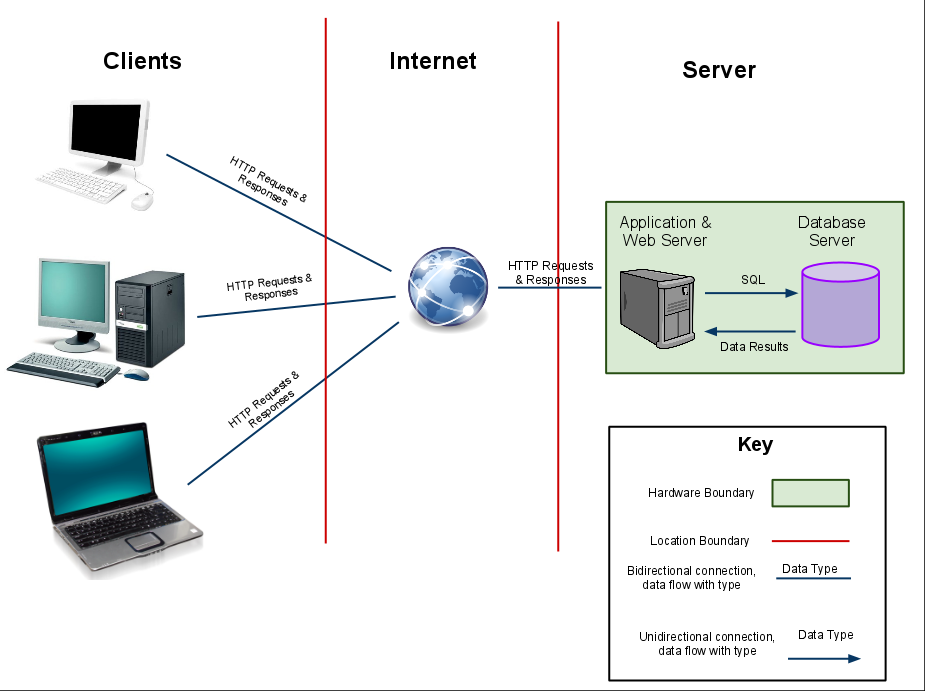
\includegraphics
			[scale=0.45]
			{images/ArchitectureOverviewDiagram.png}
		\caption{High Level Architecture Overview Diagram}
		\label{fig:aod}
	\end{center}
\end{figure}


\begin{figure}
	\begin{center}
		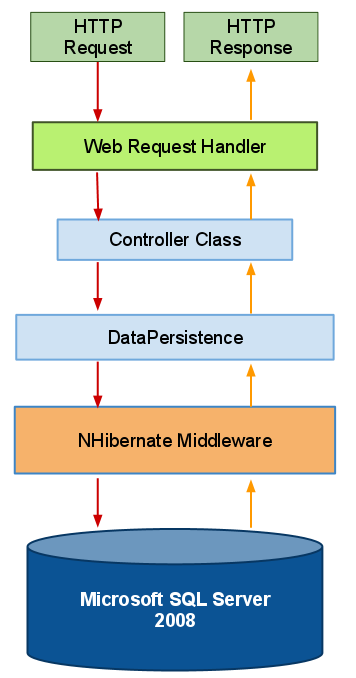
\includegraphics
			[scale=0.45]
			{images/ComponentDiagram.png}
		\caption{Diagram showing component level items}
		\label{fig:aod}
	\end{center}
\end{figure}

\section{Web Interface Design}
\label{uiDesign}
The interface design was conceptualised around the idea of a clean, consistent and intuitive interface.  It was important to ensure that Fitts' Law, the observation that the smaller a target is, the harder it is for a human to point at and act upon accurately \cite{fitts} (particularly in the 2-dimensional space of a screen \cite{fitts2d}), was taken into consideration, and a common sense approach was used when deciding how large or small clickable items should be.

Fitts' Law - 2D, clean, intuitive. Changes, suggestions from evaluators, 

\section{Class design}
This section discusses the class designs for the different versions of the program, named after NASA Space Shuttle orbiters in chronological order of when they entered service.

An \gls{oo} approach was taken with the project, as the entries that were to be saved mapped well to the concept of an object, and because the C\# language is a natively \gls{oo} language. \revisit - is this information required or relevant? % Relevant? Required?

\subsection{First model version (V0.34 - Columbia)}
The approach of the first model version was heavily based on the successful approach of Mitesh Furia; it was seen as advantageous to reuse the code from his project as much as possible, to reduce development effort and increase the output functionality at the end of this project.  With this aim in mind, the class design for the initial model was heavily structured around his approach.

The initial class design consisted of one class per entry type.  The main focus behind this approach, aside from following Mitesh's successful approach, was to take advantage of a feature of the .NET Framework called Attributes, which can be used effectively for validation.  Attributes provide the ability to associate extra information with each member variable of a class; as an example, the `required' attribute can be used to enforce the requirement to include data in a field for it to be valid.  This approach worked well for this version of the model, boasting excellent robustness to poor or erroneous user input as well as excellent feedback to users through the provision of error messages assigned by the required attribute.  Optional fields were included as normal member variables, and did not need to have attributes, aside from where their member variable name lacked spaces, resulting in poor display on the interface.  An example of a member variable name lacking spaces is the field `howpublished': it is more readable and therefore more user friendly when the field is displayed as `how published' 
Each entry type was a subclass of the abstract superclass `Publication', which contained fields common to all entry types, namely: Id, an int identifier; Cite Key, a string intended to be unique to an entry, though not necessarily in the database\revisit --- might need to mention allowance of duplicate entries here; Owner, the username of the user who created the entry in the first instance; along with Abstract, a string field which was to be optional to all entries.

As the class was designated `abstract', the enforcement of rules associated with the concept were used to the advantage of the developer: several methods, which were to be relied on and required by the controller classes, were added as abstract methods to the Publication class.  These abstract methods included two methods which converted an entry to a string representing the entry as a row in a \gls{html} table, both with and without hyperlinks to the amendment page for the entry.

Each entry type class was used directly by NHibernate and mapped by way of a Mapping class \revisit - this is implementation detail. Possibly going into too much information here, along with the discussion of the source code!

An examination of the source code\footnote{If one inspects the code for the \gls{svn} tag entitled V0.34\_Colombia, one will find that the `Publication' class contains a line commented out containing a member variable entitled (and of type) `PublicationGroup'.  This approach was not followed up, as discussed} reveals early intentions to include `PublicationGroup' as a field within Publication.  PublicationGroup was intended to be a recursively-defined structure, to allow a group to be categorised as part of a tree-based structure.  This approach was abandoned following advice from Gregg O'Malley, following his experience of trying to use very similar structures previously; his suggestion to follow a tag-based approach was noted but not acted upon until late stages of the project (see below in section \ref{designDiscovery}).

The major problem with this approach was that when it was mapped to the database by NHibernate, it resulted in one table per entry type --- 14 entry type tables in total.  The number of tables was not the biggest problem: the issue lay in the assignment of identifiers to each row and the storage of entries.  To know where to find an entry without performing a search, the system would have had to know which entry type the entry was, along with what the identifier of the entry was, as each of the entries was a weak entity.  Due to the lack of database-level guarantee that a publication's id was a unique identifier for an entry, a large refactoring took place to move all fields to one top-level table, `Publication', as discussed in section \ref{designChallenger}.
%what was wrong with it

\subsection{Second model: V1.0 - Challenger}
\label{designChallenger}
Challenger\\
Single table for all entry types:\\
why\\
what improved?\\
 - faster search\\
 - IDs all in one place - less complicated - don't need to kow what an entry's type is before searching it\\

\subsection{Third (proposed) model: V2.0 - Discovery}
\label{designDiscovery}
Discovery was intended to add a feature called `tagging' to the system.  \\
Specifically, this was to involve a many-to-many mapping from Publication to Tag


\section{DB Design Diagram}
content

%================================================

\chapter{Implementation}
\label{impl}
The implementation chapter covers the technologies, techniques and patterns applied to this project.  Many of the contents were encountered were encountered during a summer placement at a technology company in Glasgow between levels 3 and 4.  

\section{Technologies Used \& Discipline}
This section examines the technologies used in the implementation of the project and the discipline that was adhered to during development.

\subsection{Microsoft .NET Framework under C\#}
The Microsoft .NET framework is a platform for development, deployment and running of web services and applications \cite{whatIsDotNet}. This project took advantage of a particular strain of .NET, \gls{asp}.NET \gls{mvc} 2.  

Microsoft's .NET framework was used as a result of encountering the technology during the summer placement.  The developer saw the opportunity of learning more about and working with the framework when the project was successfully assigned to him.  Given that one of the aims of the summer placement was to learn .NET development, and that this aim was not achieved \cite{summerPlacementReport}, the developer chose to maximise exposure to the technology by working with it for the duration of the project, and adding an aim to learn the framework to the project goals.  It may appear that this was a short-sighted decision, but there are many other benefits to using this technology, including:
\begin{itemize}
	\item There is an active developer community on the web\footnote{The community's forums can be found at \url{http://www.asp.net/community} and a large proportion of active users of the Stack Overflow community focus on C\# and .NET topics --- 3 of the top 8 tags are directly related to the project's domain --- \url{http://stackoverflow.com/tags} (by observation)}, so issues pertaining to development using the framework can be solved by turning to this well-grounded knowledge base;
	\item The \gls{mvc} aspect of the project, if strictly adhered to by the developer, provides great separation of concerns between the place that information is stored, manipulated and viewed;
	\item The framework allows for portability to other client machines with very little in the way of model adjustment. For example, if a requirement for a mobile or tablet application developed, it would simply be a case of adding the functionality for that device, rather than having to reimplement the model for a particular piece of hardware.
	\item Applications can be deployed, with some adjustments, on Linux machines using the Mono (open source) software platform\revisit - awaiting help from Gregg
\end{itemize}

\subsection{NHibernate \& Fluent NHibernate}
\label{nhibernate}
NHibernate is a port of the Hibernate object/relational mapper to the .NET framework. In essence, it provides mapping from objects to relational tables, which allows a developer to concentrate on functionality and usability rather than spending time writing \gls{sql} scripts. Queries are generated by NHibernate middleware and passed to the database which, after execution, accumulates any results into objects directly manipulable by C\# code. 

An example of how this technology helps and works is described presently: Let's assume that a series of valid entries have been created in the database and that a user has issued a request to view the details for one of them, with the \gls{id} 3. \revisit - complete this section.


The NHibernate software itself is highly valuable in terms of time-saving potential and has been used across thousands of successful projects \cite{NhUse}.  The only issue with using it in its raw form is that mappings from the project's classes to relational entities have to be written in \gls{xml}, a language prone to errors often left unnoticed until runtime.  A better solution is to use the Fluent NHibernate extension, which provides developers with the ability to map the classes in code.  The major benefit of this scheme, aside from compile-time error checking, is that all code using is strongly-typed; combine this with the powerful \gls{msvs} \gls{ide}, and implementation for the data model can be quite rapid --- particularly when in the hands of an experienced developer.

Another reason for using this technology was that it was used within the summer placement, but it was not encountered or worked with to any great extent.  \revisit Curiosity fuelled, the developer wanted to expand his knowledge in the technology in both breadth and depth by adopting these technologies within the project.

There was a risk, when employing this technology, that unfamiliarity would lead to hindrance rather than benefit by employing it.  Before automatic generation of database scripts for interactions can take place, Fluent NHibernate has to be instructed what to map and how to map it.  This was not something that the developer had encountered before; the risk was that learning how to map the classes to entities correctly would take too much time and have an impact on the progress of the project.  To mitigate the impact of the risk, a deadline was agreed between the developer and the supervisor: if, by the final day of term in semester 1, the mappings were not working correctly, then NHibernate as a data solution would be abandoned and standard \gls{sql} queries would be used.  As it turned out, the mappings were finalised on the afternoon of the deadline, so NHibernate use went ahead.  The aforementioned benefits of NHibernate were noticed during development, and some experience was gained in the implementation and use of object/relational mapping in practice.

\subsection{Subversion}
\label{svn}
\gls{svn} is a centrally-stored version control system which records every change ever made to the files and directories in the file repository \cite{CFP04c1}.  It is useful to be able to centralise the code repository and to be able to synchronise different workstations with the most up to date version of code and documents, as well as allowing the logging and comparison of different versions of the code.  Each time information is updated in the repository, it is said to have a new revision -- a process also known as `committing' changes.  It was decided early in the project that a repository would be used to mitigate the risk of fire, flood, theft, and hard drive corruption by hosting the repository in a different physical location to the main work environment, the developer's laptop.  

\gls{svn} was used to control different versions of the code and to take snapshots of the project in the form of \gls{svntag}s \cite{CFP04c4}, as well as normal revisions.  It was originally hosted on the School of Computing Science network because it was accessible from outside the School's network of computers\footnote{access was facilitated by the School's \gls{ssh} gateway, \texttt{sibu.dcs.gla.ac.uk}}, because there was sufficient storage space provided by the School and it had no financial cost.  As part of the effort to ensure good software engineering practice, \gls{ci}\footnote{See Section \ref{continuousIntegration} for an explanation of what it is and why it was used} was to be used with the project, again after encountering it while on summer placement.  Unfortunately, there were problems in configuring the  \gls{ci}  software to access the \gls{svn} repository through the gateway; as a result of this, on the 16\^{th} of November 2010, the repository was moved to another free host, SourceForge, an open-source software project hosting provider.  Along with \gls{svn} repository hosting, SourceForge provides tools for management of software projects, including a bug tracking tool (see Section \ref{bugTracking}).  Crucially, the SourceForge repository was accessible by the \gls{ci} software, allowing the \gls{ci} process to take place.

The \gls{svn} client in most cases was TortoiseSVN, as development was to take place on a windows environment.  AnkhSVN, a secondary client, was also used as it integrated with the \gls{msvs} \gls{ide}. 

The change log from the \gls{svn} repository is included as an appendix\revisit; the repository can also be browsed on the SourceForge website at \url{http://bibman.svn.sourceforge.net/}

\subsection{Bug Tracking}
\label{bugTracking}
Bug tracking is, as the name suggests, the tracing of the status of bugs that have been discovered in a system, used primarily to ensure that bugs which are found are dealt with or logged in a release.  It is another concept that was encountered while on summer industrial placement, and it struck the developer as an advantageous \gls{case} tool to utilise in this project.

The bug tracker was used when a bug was encountered that was not going to be fixed at the time of the discovery; the developer wanted to apply use of the bug tracker intelligently so that it was always going to be a help, and not a bureaucratic hindrance to development.  Bugs that were found were created in the system and given a priority, marked initially as `open' to symbolise that they had not yet been dealt with.  When a bug had been dealt with and the developer had verified that it was no longer an issue, it was marked as `closed', and remained in the system for traceability, should a similar issue crop up.  As a rule of thumb, a comment was recorded to say firstly what the problem was, secondly what the fix was and thirdly which \gls{svn} check-in fixed the issue so that one did not need to trawl through logs in \gls{svn} to find the fix, should they need to revisit it.\\ \revisit - want to check wording of this paragraph when I'm not tired.

The software used was BugTracker.NET -- a free, open-source, web-based bug tracker.  Having encountered this particular product and worked with it for three months, the developer thought it wise to stick to familiar ground and employ the same product.  The developer used hardware running at home to deploy BugTracker.NET and used it until a server failure in late January 2011.  As the hardware was no longer reliable to host the software, the decision was taken to switch bug tracking software to SourceForge's Bug tracker, which worked in a similar way.  Bugs from the old system (both open and closed) were transferred to the new site and remain there now for traceability and reference. \\

\section{Development Environment}
\label{deveEnv}
Most development took place on the developer's laptop, a MacBook Pro dual-booted with Windows 7 Professional.  Development also took place on a second developer machine when the laptop was unavailable.

The main development environment was Microsoft's Visual Studio Professional 2010 (\gls{msvs}), provided by the School's \gls{msdnaa} agreement.  This was the same environment used while on summer placement, so the developer was familiar with the tools in the \gls{ide}.

The database product used was \gls{msss} 2008 Developer Edition, again provided by the School's \gls{msdnaa} agreement. The management suite included with the product was again used while on summer placement, and the developer was familiar with the tools in the program.

ReSharper is a productivity plug-in for \gls{msvs}.  It provides code inspections, code analysis, one-click unit test runs, project-level refactorings and many more assistive features. A licence for the product was bought during the summer placement and was used extensively throughout the development of the software article.

Python IDLE and Notepad++ were used to manipulate code quickly and effectively: Python IDLE for its scripting functionality and Notepad++ for its macro capabilities and excellent search and replace by regular expression function.

TortoiseSVN and AnkhSVN were both used as discussed in section \ref{svn}.

\section{Reuse of Code}
\label{codeReuse}
ADV:
Code reuse within project \\
Code reuse from other projects \\
 - pre tested
 - see somerville for more info.

Benefits of code reuse:
\begin{itemize}
	\item the reduction of maintenance overheads of having to test the same code in multiple places
	\item 
\end{itemize} 

Disadv/risks:
	bugs may exist if not widely used or well tested
	code may be less readable if not familiar with it
	

\section{Patterns}

% reset mvc acronym.
\glsreset{mvc}
\subsection{Model View Controller}
The application is heavily based on the \gls{mvc} architecture.  The data model and database interaction is all taken care of in core classes, namely the \texttt{DataPersistence} and \texttt{Publication} classes.



\section{Data Model}
Discuss implementation of data model, implementation of database persistence. centralised persistance information - single section of code + benefits.
The data model, as mentioned in section \ref{nhibernate}, is implemented using NHibernate.  
Discuss fields in publication table. Mention creation/modification/deletion times and what they are used for
ID field vs cite key
owner


\subsection{Refactoring}
changes to model from 0.34 to 1.0


\section{Controller}
Home controller
Account Controller
Entry controller:
 - Same page for add and amend
 - discuss import
 - 
Discuss handling of requests


\section{Web Service}
Delete by AJAX\\
search\\
'what is new'\\
'what is amended'\\
'what is deleted'\\




\section{View}
\glsreset{ui}
\subsection{Consistency}
The consistency sought in the design of the product (see section \ref{uiDesign}) of the site is a result of careful consideration of what should be consistent across all pages, as highlighted in figure \ref{fig:pageLayout}:

\begin{figure}
	\begin{center}
		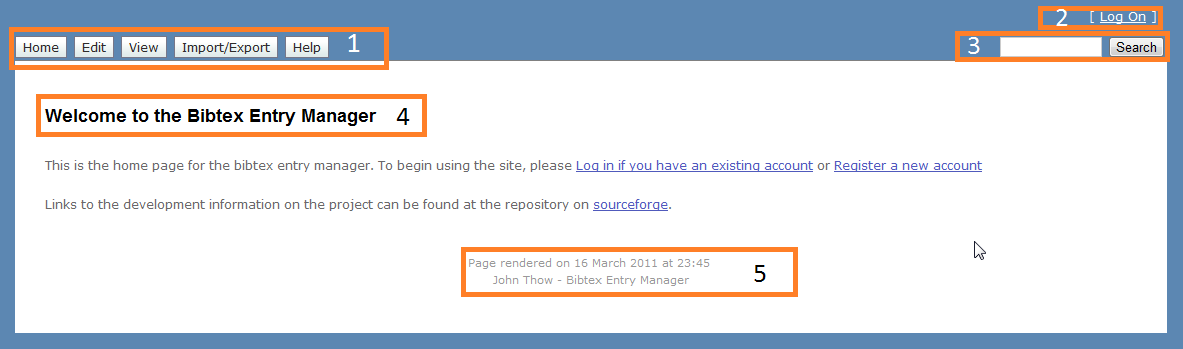
\includegraphics
			[scale=0.5]
			{images/PageLayout.png}
		\caption{Annotation of a page}
		\label{fig:pageLayout}
	\end{center}
\end{figure}

\begin{figure}
	\begin{center}
		
\includegraphics
			{images/LogOff.png}
		\caption{The log on area when a user is logged in (swapped out for area 2 in figure \ref{fig:pageLayout})}
		\label{fig:logOff}
	\end{center}
\end{figure}

\begin{enumerate}
	\item Firstly, there is a menu area which appears on every page within the site, with the same options at each appearance.  This gives the user a single point of reference to aid navigation of the website \revisit - cite someone
	\item The log on area appears in one of two forms across all pages of the application: a user is either browsing anonymously, or is logged in.  It is clear which of these two states the user's session is in thanks to the clear representation of the words `Log On' (depicted in figure \ref{fig:pageLayout}) and a welcome message with the current user's email address (as depicted in figure \ref{fig:logOff})
	\item After feedback from a user during the basic evaluation (see Chapter \ref{eval}) the interface was updated to include a search area on all pages.  The provision of this area allows a user to efficiently search the system's database for a string and, by making it a consistent feature, gives another concrete point of reference across all pages.
	\item Each and every page contains a bold header indicating the title of the page.  The presence of a title on each page gives a user another concrete and consistent place to glance in order to gain an insight into what they previously clicked on, as well as giving confirmation that their previous action was successful.
	\item The fifth item highlighted in this image provides some extra, arguably unnecessary information.  The main idea behind including this page render time area is to provide extra feedback: it lets a user know that page has finished loading, that it has been completed successfully and it reassures a user that the page is up to date.
\end{enumerate}

This consistency was implemented using a feature in \gls{asp}.NET called Master Pages.  As the name suggests, the developer creates a master page with the main layout of the website, within which sit containers which are filled by individual pages.  This approach centralises the code for the pages, the advantages and disadvantages of this are discussed in section \ref{codeReuse}. \revisit revisit fluency.

The colour choice of the interface was a decision which was postponed until later in the project, so that the bulk of the development work could be carried out before aesthetics were considered.  The colour scheme seen in the project is heavily based on the default style for projects created in \gls{msvs} 2010; it soon became apparent that the default style had many strong qualities that could be used 

\section{Concurrency}

%================================================

\chapter{Testing}
\label{testing}
Dijkstra is often quoted as saying ``testing can only prove that errors are present, not that they are absent'' \cite{dijkstra}. This is true, but it is also the case that effective validation of a software product increases the confidence that a software product acts as it is supposed to.  This section of the dissertation is intended to convey information about the testing of the application, to increase the reader's confidence in the in the system and to convey information about the software engineering practice that was applied during testing.

\section{Unit Testing}
A unit test is a test on a unit of code in isolation: a comparison of the actual result of an operation with its expected output \cite{unitTesting}.  A series of unit tests can (and should) be run frequently to ensure that changes to code have not resulted in the development of problems elsewhere.  A unit test comprises of four main areas of execution:
\begin{itemize}
	\item Set up -- the set up phase ensures that any prerequisites for the test are set up before the test begins, for example a session with a database;
	\item Act -- the phase where the unit of work under test is executed on the target object(s);
	\item Assert -- the comparison between the expected result and the actual result.  If the two do not match for a test (or an unexpected exception is thrown) it is said to have failed the test and if expected and actual results are the same, it is said to have passed;
	\item Tear down -- after each and every test, a tear down must occur.  Often, this is just a case of allowing the garbage collector to deal with unused objects, but sometimes connections to databases, file sessions and other connections must be closed.
\end{itemize}

% NUnit - what, why, how.
NUnit is an open source unit testing framework for the .NET languages, originally ported from the unit testing framework for Java, JUnit \cite{nUnitHome}.  NUnit 2.5.7 is used within the project and was the most up-to-date version at the beginning of project development (released in August of 2010 \cite{nUnitRelease}).  

NUnit allows unit tests to be written as methods in a class, which can be run inside or outside the \gls{msvs} \gls{ide}, through ReSharper (see section \ref{devEnv}), which allows one-click running of unit tests and sets of unit tests.

\section{Continuous Integration}
\label{continuousIntegration}
Continuous Integration is a technique which minimises the risk of bugs cropping up between \gls{svn} revisions.  It works by automatically performing a build then running all unit tests each time a revision is committed to the repository, meaning that if issues arise between versions, they are noticed early and can be dealt with as and when they crop up.  There are several stages in setting up this process, as laid out by Martin Fowler in his paper on Continuous Integration \cite{fowlerCI}.  The important points are outlined below, but for the full picture (an approach particularly aimed at teams of developers), see Fowler's article:
\begin{enumerate}
	\item A single source repository must be used.  This was achieved as laid out in section \ref{svn};
	\item The build must be automated.  This was achieved by bundling a command into a \gls{bat} script, which can in turn be run from the command line or the Windows Explorer interface.  This script used Microsoft's \texttt{msbuild} program, which uses an \gls{xml} file to organise how a build should take place, much like the way a \texttt{makefile} can be used in \gls{unix}-based operating systems;
	\item The build must be self-testing: tests are included as part of the \gls{xml} file mentioned in the previous step, which means that when the \gls{bat} file is run, all of the tests associated with the solution are executed on the freshly built executable.  This means that any bugs that crop up since the last build can be found and dealt with early, saving development and maintenance time later on;
	\item Every commit should build the mainline on an integration machine. In essence, this point is trying to ensure that the build and the test for the \gls{ci} cycle take place on a separate machine from the main development environment, ensuring that the project is not dependent on files left on the developer's machine --- in effect, this means that the \gls{ci} software must run on another computer.  This was achieved by using separate hardware from the developer machine, running \gls{ci} software called CruiseControl.NET (discussed below).  
	\item The developer is notified as soon as the build has finished, by way of a pop-up in the notification area of their computer.  Any issues can be fixed as soon as they arise, rather than being discovered further down the development line.
\end{enumerate}

CruiseControl.NET is an open-source program from Fowler's employer, ThoughtWorks, which acts as a monitor to the repository: it automatically checks-out code each time a commit takes place, builds the project and then runs all unit tests, before outputting the result of the build to both a web page and the CruiseControl Notification Tray client. \revisit - include screenshot of both

The \gls{ci} cycle is primarily intended for teams of developers. \gls{ci} leads to a `Test Early. Test Often. Test Automatically.' attitude --- it drives the developer to find find bugs now, which helps to avoid users finding bugs later \cite{pragmaticProgrammer}. Risks associated with deferred integration (integration after a long time or large numbers of changes, antonymous to continuous integration), which include .



CruiseControl.NET - what, why, how. Take from SE placement info to save time + effort \cite{fowlerCI}

\begin{figure}
	\begin{center}
		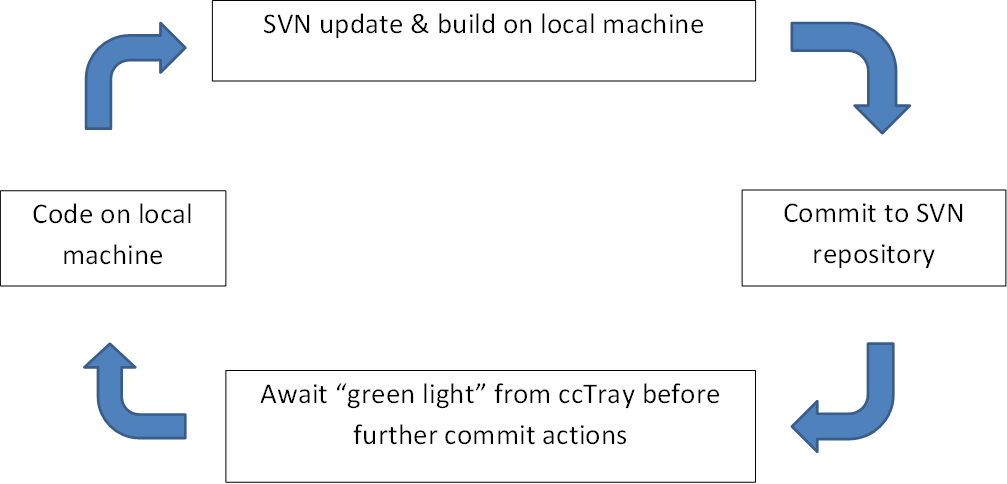
\includegraphics
			[scale=0.5]
			{images/ContinuousIntegration.png}
		\caption{The CI Cycle}
		\label{fig:continuousIntegration}
	\end{center}
\end{figure}

\section{Bug Tracking}


\section{Acceptance Test}
For the project to pass the acceptance test, all unit tests associated with the project must pass.  By the end of the project, there were \revisit unit tests, all of which passed.

%================================================
\chapter{Evaluation}
\label{eval}
This chapter discusses the evaluations that were carried out on the project.  In particular, it discusses the ... \revisit \\

It was decided that any evaluation of the system would be short-sighted and ineffective without the assistance of people who had not been previously involved in development of the project, as an insider might not be able to provide a completely impartial examination of the system. \revisit

\section{General Approach}
The evaluation took two forms: firstly, a basic usability evaluation, focussing on a single user's interactions with the system; and secondly, an extended evaluation, examining the positive points and shortcomings of the system when multiple users were working with the system.

It was hoped that a sample of users external to the project, with various levels of knowledge of \bibtex \& \LaTeX, would participate in the study. The intention of sampling a range of users' views ensured that the evaluation would gain a fair set of opinions on the product for analysis, so that the evaluation had as wide a set of views on the product as possible. 

As the evaluation would involve other people, the `School of Computing Science Ethics Checklist'\footnote{The signed ethics checklist document is included as an appendix to this document.} was consulted to ensure that the intended evaluation was ethically sound and that it would not put participants at any greater risk than they encounter in their normal working lives.

The evaluations had slightly different environments, which will be discussed within the relevant sections below.  The different evaluations are explained, and have their results included with each 

\section{Basic Usability Evaluation}
The basic usability evaluation is based around the points raised in the background survey (chapter \ref{backgrnd}).  Recall that the examination criteria in the background survey were centred around the \gls{ui} to the system, the features of the system and how fault tolerant \& robust the system was.

\subsection{Environment}
Laptop with mouse, connected to the internet.\\
The participant sat at a desk on an adjustable-height chair in a well-lit, quiet room at a comfortable temperature.	Room 620 in the Boyd-Orr Building was the location for some of the experiments, while others took place \revisit \\
Is this part necessary? Need to say why the environment was important - focus on task at hand, no discomfort while participating etc?

\subsection{Execution}
The following terminology is used consistently throughout this section: the `participant' means a volunteer who participated in an evaluation of the system and the `host' means the person who was running the evaluation; in all cases, the host was the developer of the system.\\
Completed evaluations were structured as follows:
\begin{enumerate}
	\item The host presented the participant with introduction script;\footnote{Introduction and debrief scripts are included as appendices to this document}
	\item The participant read introduction script;
	\item The host asked the participant to verbally confirm that they agreed to take part in the evaluation;
	\item The participant agreed to take part;
	\item The participant was asked to familiarise themselves with the system by using the site for as long as they wished, and was encouraged to ask questions of the host;
	\item The participant told the host that they were ready to proceed;
	\item The host cleared the system and presented the participant with the task list\footnote{The task list is included as an appendix} and any points that the participant raised while performing tasks were noted by the host; \revisit Should I mention that the URL for the import task was http://toms.acm.org/Volumes/V37.html?searchterm=bibtex
	\item The participant told the host that they had completed the task list;
	\item The host gave the participant a questionnaire, which they filled in. Notes taken by the host on the participant's behalf were given to them to remind them of things they had mentioned;
	\item The participant gave the host the completed questionnaire, which was put into an opaque folder in a random order, to help preserve participants' anonymity;
	\item The host gave the participant the debrief script;
	\item The participant took a note of the email addresses provided and was given a final chance to ask questions during the evaluation;
	\item The host thanked the participant for their time.
\end{enumerate}

While the participant was performing tasks, the host noted relevant points that the participant raised.  This was done in an attempt to help the participant to focus on the task at hand, rather than leaving the participant to recall the comments they made; it also allowed the host to gain a better insight into any difficulties encountered by the participant.

\subsection{Results}
Tabulate results from the evaluations and go on to analyse the results.

\subsection{Analysis}
Sample of users - some CS students targeted, Physics/Astronomy students, staff \& users who don't have academic knowledge - relevant point? why use them? Worth mentioning at all?

\section{Extended Usability Evaluation}

\subsection{Environment}
\subsection{Execution}
\subsection{Results}
\subsection{Analysis}

\section{Summary of Evaluations}

\subsection{Potential Improvements to Evaluations}


%================================================

\chapter{Conclusion}
\label{conclusion}

\section{Summary}

\section{Suggestions for Further Work}

\appendix
\printglossaries

\bibliographystyle{plain}
\bibliography{l4proj}
\end{document}
